\chapter{Introduction}

This report is part of the final submission for the course \emph{Sustainable Computational Engineering}, held by Dr. Anil Yildiz and Dr. Hu Zhao of the \emph{Chair of Methods for Model-based Development Methods in Computational Engineering} \cite{mbd}. The aim of this course is to learn about sustainable and reproduceable model development practices, data life cycles, and data visualization. For the final assignment, each participant is supposed to implement a Python package that showcases some aspect data-driven modelling or visualization while being useful in the context of their own research interests or work.

In my final project, I chose to implement a Python package for interactive visualization of volumetric images and segmentations. My personal research interest is biomedical imaging, more specifically the analysis of computed tomography (CT) scans. The package I implemented is called \emph{slicevis} (think: slice visualization) and it is publicly available on PyPI \cite{slicevis}.

\begin{figure}[h!]
	\centering
	\begin{subfigure}[t]{0.45\linewidth}
		\centering
		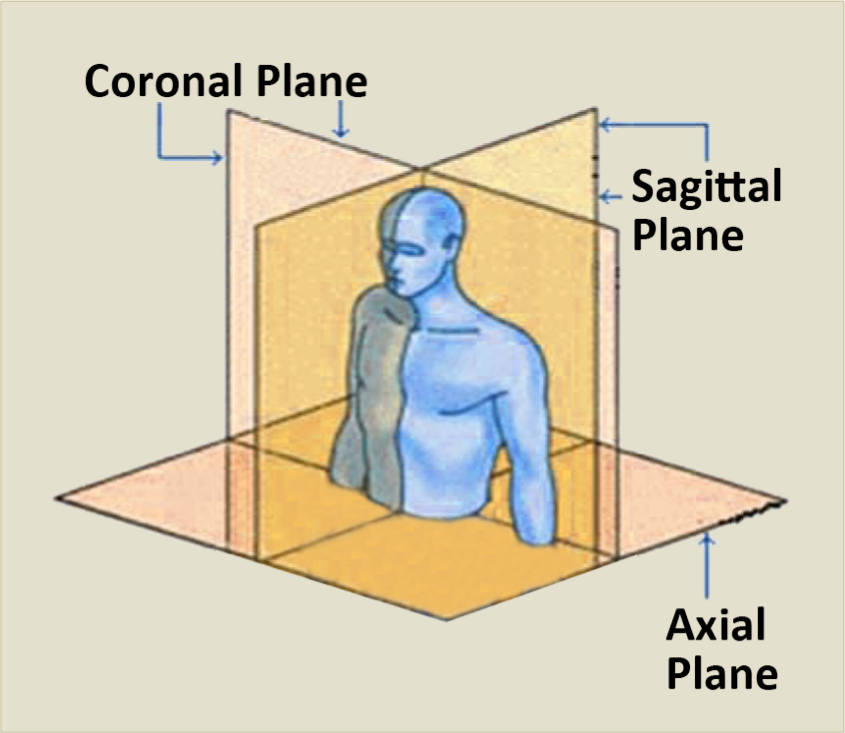
\includegraphics[width=\linewidth]{figures/slices.png}
		\caption{Axial, coronal, and sagittal plane of body \cite{slices}.}
		\label{fig:slices}
	\end{subfigure}
	\hfill
	\begin{subfigure}[t]{0.45\linewidth}
		\centering
		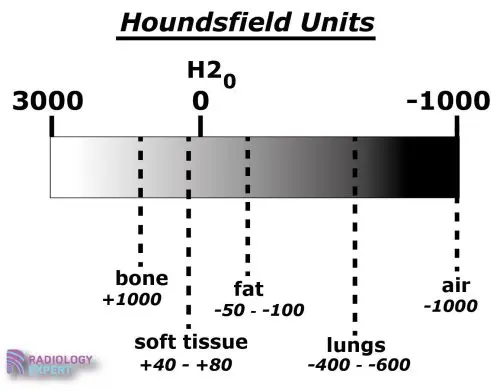
\includegraphics[width=\linewidth]{figures/hounsfield.png}
		\caption{The Hounsfield scale \cite{hounsfield}.}
		\label{fig:hounsfield}
	\end{subfigure}
\end{figure}

The term \emph{slice} refers to a two-dimensional image that represents a cross-section of a three-dimensional image along one of the axes. In the field of biomedical imaging, there is a naming convention for \emph{axial, coronal, } and \emph{sagittal slices}. This is illustrated in \cref{fig:slices}. 


CT scans are used in practice to diagnose a wide variety of medical conditions \cite{ct}. Most commonly, the upper body is scanned to analyze the lungs or the heart. As CT relies on ionizing radiation (X-rays) to create volumetric images, it is not entirely risk-free. Image quality generally varies with the so-called \emph{voxel size} which is typically less than one millimeter. One very useful aspect about CT images is that the scanners are calibrated to the Hounsfield scale. Hence, one can directly infer from the intensity values in the image to the tissue type, as shown in \cref{fig:hounsfield}. This greatly aides in segmenting the data into classes such as foreground/background, major organs and the skeleton. 

There are three following chapters in this report, namely \emph{Package Structure, Implementation,} and \emph{Use-Cases}. The second chapter describes all aspects of the repository for \emph{slicevis} as it is also part of the final submission. In \emph{Implementation}, I will go into detail about the Python code. Lastly, three use-cases are described which illustrate how \emph{slicevis} can be useful in the context of biomedical research.
